\documentclass[tcc-proposta]{texufpel}

\usepackage[utf8]{inputenc} % acentuacao
\usepackage{graphicx} % para inserir figuras
\usepackage[T1]{fontenc}
\usepackage{array}

\hypersetup{
    hidelinks, % Remove coloração e caixas
    unicode=true,   %Permite acentuação no bookmark
    linktoc=all %Habilita link no nome e página do sumário
}

\unidade{Centro de Desenvolvimento Tecnológico}
\curso{Ciência da Computação}
\nomecurso{Bacharelado em Ciência da Computação}
\titulocurso{Bacharel em Ciência da Computação}

\title{Plataforma Web para Monitoramento de Dados Oriundos de Redes de Sensores sem Fio}

\author{Huber}{Mathaus Corrêa}
\advisor[Prof.~Dr.]{Marques}{Felipe de Souza}
\coadvisor[Prof.~Dr.]{Corrêa}{Ulisses Brisolara}
%\coadvisor[Prof.~Dr.]{Aguiar}{Marilton Sanchotene de}
%\collaborator[Prof.~Dr.]{Aguiar}{Marilton Sanchotene de}

\begin{document}

%\renewcommand{\advisorname}{Orientadora}           %descomente caso tenhas orientadora
%\renewcommand{\coadvisorname}{Coorientadora}      %descomente caso tenhas co-orientadora

\maketitle 
\sloppy

\chapter{Dados de Identificação}

\section{Nome do Projeto}
Plataforma Web para Monitoramento de Dados Oriundos de Redes de Sensores sem Fio

\section{Local de Realização}
Centro de Desenvolvimento Tecnológico (CDTec)/Universidade Federal de Pelotas (UFPel)

\section{Responsável pelo Projeto}
Mathaus Corrêa Huber

mchuber@inf.ufpel.edu.br

\section{Professor Orientador}
Prof. Felipe de Souza Marques

\section{Professor Co-orientador}
Prof. Ulisses Brisolara Corrêa

\chapter{Sumário Executivo}
% (NO MÁXIMO 1 PÁGINA)
Embora a ideia de IoT já exista há muito tempo, uma série de avanços tecnológicos recentes em algumas áreas tornou-a possível em termos práticos. Com esse conceito, através dos dados gerados podemos transformá-los em informação valorável para os seres humanos com a conectividade de dispositivos usando a internet como canal comum.
\\

Dessa forma, este trabalho detalha o desenvolvimento de uma aplicação web capaz de apresentar informações estruturadas a partir de \textit{dashboards}, que consideram dados oriundos de diferentes tipos de Redes de Sensores sem Fio (RSSF) aplicadas a \textit{smartfarms}, \textit{smartcities}, \textit{smartcampus}, etc. A plataforma disponibilizará APIs para os usuários cadastrados, permitindo a configuração de um \textit{dashboard} para monitorar dados de diferentes tipos de sensores, incluindo a possibilidade de monitoramento de dados de telemetria. A partir da disponibilização destas funcionalidades em uma plataforma web, almeja-se garantir um fluxo constante de dados, que darão origem a séries históricas para que sejam realizadas análises preditivas. \\

Inicialmente, a plataforma será validada a partir de dois estudos de caso, envolvendo uma aplicação rural para o manejo integrado de pragas e outra para o monitoramento de estações hidrológicas e meteorológicas espalhadas no entorno da bacia da Lagoa Mirim. O objetivo da validação será testar a integração e confiabilidade do sistema. Estas aplicações foram escolhidas pois as soluções de monitoramento estão sendo desenvolvidas em projetos do grupo de pesquisa em que o proponente está inserido, o que garantirá acesso aos sensores das RSSFs.



%Apresentar aqui uma breve Introdução ao Problema que está se
%pretendendo resolver ou abordar. Além disso, nesta seção,
%apresenta(m)-se o(s) principal(is) objetivo(s) do projeto e, portanto,
%a(s) principal(is) contribuição(ções)~\citet{Moore:1979:MAI,Aguiar:2005}.

\chapter{Histórico e Justificativa}
% (NO MÍNIMO 1 PÁGINA)
Atualmente, um dos assuntos em alta na área de tecnologia é justamente a Internet das coisas, que se tornou uma das tecnologias mais importantes do século, ao proporcionar a conexão de objetos do cotidiano à Internet, por meio de dispositivos incorporados entre a comunicação de pessoas e processos. \citet{Almeida:2015} se refere à Internet das Coisas como a integração de objetos físicos e virtuais em redes conectadas à Internet, permitindo que “coisas” coletem, troquem e armazenem uma enorme quantidade de dados na nuvem, em que uma vez processados e analisados esses dados, geram informações e serviços em escala inimaginável. Conectando a ideia de IoT a um sistema de informação, mais especificamente um sistema web, executando diretamente na internet.
\\

Segundo \citet{O’BRIEN:2013} um sistema de informação é definido como “uma
combinação organizada de pessoas, hardware, software, redes de comunicação, recursos de dados e políticas e procedimentos que armazenam, restauram, transformam e disseminam informações em uma organização". Com isso, visando unir o mundo físico e o virtual, conectando a tecnologia IoT ao setor do agronegócio, aplicando um conceito de \textit{smartfarm}, este trabalho busca trazer um software web, que nada mais é do que um sistema de informação projetado para utilização dentro de um navegador, disponibilizando assim menor custo de manutenção e escalabilidade.
\\

Cabe destacar que, o agronegócio é considerado um dos setores mais importantes da economia do país e possui um grande potencial de crescimento. Alcançando níveis recordes do produto interno bruto brasileiro em 2020, representando cerca de 26,6\% do Produto Interno Bruto – PIB
do país, sendo considerada uma das áreas mais importantes para os economistas no país atualmente. \citet{Cepea:2021}
\\
%Visando unir o mundo físico e o virtual, conectando a tecnologia IoT ao setor do agronegócio, área extremamente aquecida no cenário global atualmente. Este trabalho busca trazer uma plataforma que agrega uma tecnologia de sensores de baixo custo e baixa potência conectados a uma série de protocolos em rede para uma aplicação web.

Contudo, a realidade nem sempre foi essa, segundo um estudo da Empresa Brasileira de Pesquisa Agropecuária (Embrapa), publicado por ~\citet{Schuh:1971}, no século passado, a agricultura no país era predominantemente rudimentar, contando com menos de 2\% das propriedades rurais com acesso à máquinas agrícolas. Nesse âmbito, a produção pecuária no final da década de 1950 se configurava como uma das mais baixas do mundo, e produções como a soja ainda eram vistos como uma inovação pouco alcançável para os parâmetros da época. 
\\ 

De acordo com \citet{Canuto:2012}, para auxiliar o produtor na forma como gerencia e administra sua
propriedade, surgiram as inovações tecnológicas. Partindo desse princípio, investir em tecnologias e inovações para o setor se torna cada vez mais necessário, uma vez que, com o avanço dos sistemas digitais podemos torná-lo ainda mais competitivo, entregando bons resultados e promovendo um ambiente de crescimento mais valorável.
\\

%Dessa forma, levando em consideração o grande potencial, em termos econômicos, do setor do agronegócio, almejamos trazer um sistema de monitoramento de pragas que contam com a utilização de sensores que entendem o ambiente e enviam os dados para uma plataforma única centralizada. 

Mesmo sabendo a existência de ferramentas e estratégias para o auxílio à tomada de decisão no agronegócio, uma das grandes complicações muitas vezes se dá devido à dificuldade no manejo da tecnologia por parte dos produtores rurais. Na área de tecnologia é muito comum a adaptação e implementação de técnicas que foram desenvolvidas por outros à nosso contexto. A exemplo disso, \citet{Valter:Lucas:2019} propôs uma abordagem através de Redes Neurais Convolucionais para identificação de duas espécies de moscas-das-frutas, que possivelmente pode vir a ser usado como uma estratégia para reconhecimento de outras espécies de pragas dentro do trabalho este que está sendo proposto.
\\

Nota-se que, embora seja uma plataforma de auxílio e tomada de decisões para o produtor rural, o uso de métodos de Inteligência Artificial para utilização de modelos de predição com base nos dados gerados pelos sensores em campo pode auxiliar o produtor a entender a ocorrência de determinada praga e evitar infestações. 
\\
%muitas vezes, devido à heterogeneidade das propriedades rurais, não atendem as reais necessidades dos produtores. A dificuldade de apropriação de um software de gestão em pequenas propriedades rurais é outro fator que distancia os agricultores dessa tecnologia, geralmente por não conhecer os benefícios das Tecnologias da Informação e Comunicação (TIC) e não saber operá-la

Atualmente, os sistemas de informação também são de grande importância para o monitoramento de recursos hídricos. O uso dos recursos hídricos de rios por meio de reservatórios e barragens é de fundamental importância para a geração de energia, abastecimento de água, navegação, agricultura e controle de inundações. Mais da metade dos principais sistemas fluviais do mundo possuem reservatórios represados, que controlam ou afetam o fluxo de um determinado rio \citet{Joo:2015}. Logo, a gestão destes reservatórios de água é um problema crítico, pois a previsibilidade do nível da água é relevante para avaliar problemas estruturais em barragens, garantir o abastecimento de água e disponibilidade de recursos, garantir a qualidade da água, conservar a biodiversidade, viabilizar a navegação, prevenir desastres e otimizar da produção de energia hidrelétrica.
\\

O Núcleo de Ensino, Pesquisa e Extensão em Hidrometria e Sedimentologia para o Manejo de Bacias Hidrográficas \citet{hidrosedi:2022}, da UFPel, realiza o monitoramento do nível e qualidade da água da bacia da Lagoa Mirim, incluindo a Barragem Eclusa do Canal São Gonçalo, localizada em Pelotas no Rio Grande do Sul. Diferentes sistemas de hardware e software são utilizados e uma das necessidades do grupos é ter um sistema integrado para o monitoramento de diferentes grupos de sensores. Além disso, também seria de extrema relevância a possibilidade de prever o nível da água, especialmente no jusante e montante da Eclusa.
\\

As aplicações descritas acima demonstram que podem ser beneficiadas por sistemas de informação mais robustos. No caso das aplicações voltadas à \textit{smartfarms}, alguns softwares ou sistemas de informação podem ser comparados à proposta deste trabalho. O que mais se assemelha é o \citet{farmbox:2022}, desenvolvido para monitoramento e gestão do campo. Esta solução não apresenta nenhum tipo de funcionalidade para realizar análises preditivas. De forma semelhante, as soluções utilizadas pelo NEPE-HIDROSEDI não estão integradas em um único sistema. Além disso, nos dois casos, são soluções proprietárias fechadas, que dificultam o acréscimo de funcionalidades, que podem ser úteis para projetos de pesquisa que visam o desenvolvimento de novas tecnologias.
\\

De forma a propiciar um sistema integrado para o monitoramento de dados de diversos sensores, este trabalho propõe o desenvolvimento de uma plataforma web que viabilizará a conectividade dos sensores por meio de APIs, que concentrarão seus dados em uma base de dados única. A partir desta integração, pretende-se desenvolver metodologias para realizar análises preditivas, através de técnicas já conhecidas de aprendizado de máquina, ou até mesmo de aprendizado profundo. A plataforma desenvolvida será validada junto aos sistemas utilizados pelo NEPE-HIDROSEDI e em uma aplicação voltada ao manejo integrado de pragas, que está sendo desenvolvida em projetos de pesquisa do grupo de Pesquisa em Engenharia de Sistemas Ciber-Físicos da UFPel em parceria com empresas locais.  
%Nesta seção, apresenta-se um breve histórico da área de concentração
%do Projeto, partindo do tema mais abrangente até chegar
%especificamente no assunto do Projeto. Além disso, apresenta-se a
%justificativa para a realização do trabalho, sua importância acadêmica
%ou para comunidade e grau de inovação. Poderá também apresentar as
%distinções entre o trabalho atual e outros trabalhos já
%realizados~\cite{vonNeumann:1966:TSR}.

\chapter{Objetivos e Metas}
Este trabalho tem como objetivo desenvolver uma plataforma web para fornecer \textit{dashboards} e APIs, voltada à internet das coisas aplicadas a \textit{smartfarms}, \textit{smartcities}, \textit{smartcampus}, entre outros. A API criará um camada abstrata para monitorar dados de diferentes tipos de sensores, incluindo a possibilidade de monitoramento de dados de telemetria. Como objetivo secundário, almeja-se garantir um fluxo constante de dados, que darão origem a séries históricas permitindo o desenvolvimento de modelos para análises preditivas. 
\\

\begin{figure}[!htb]
    \centering
    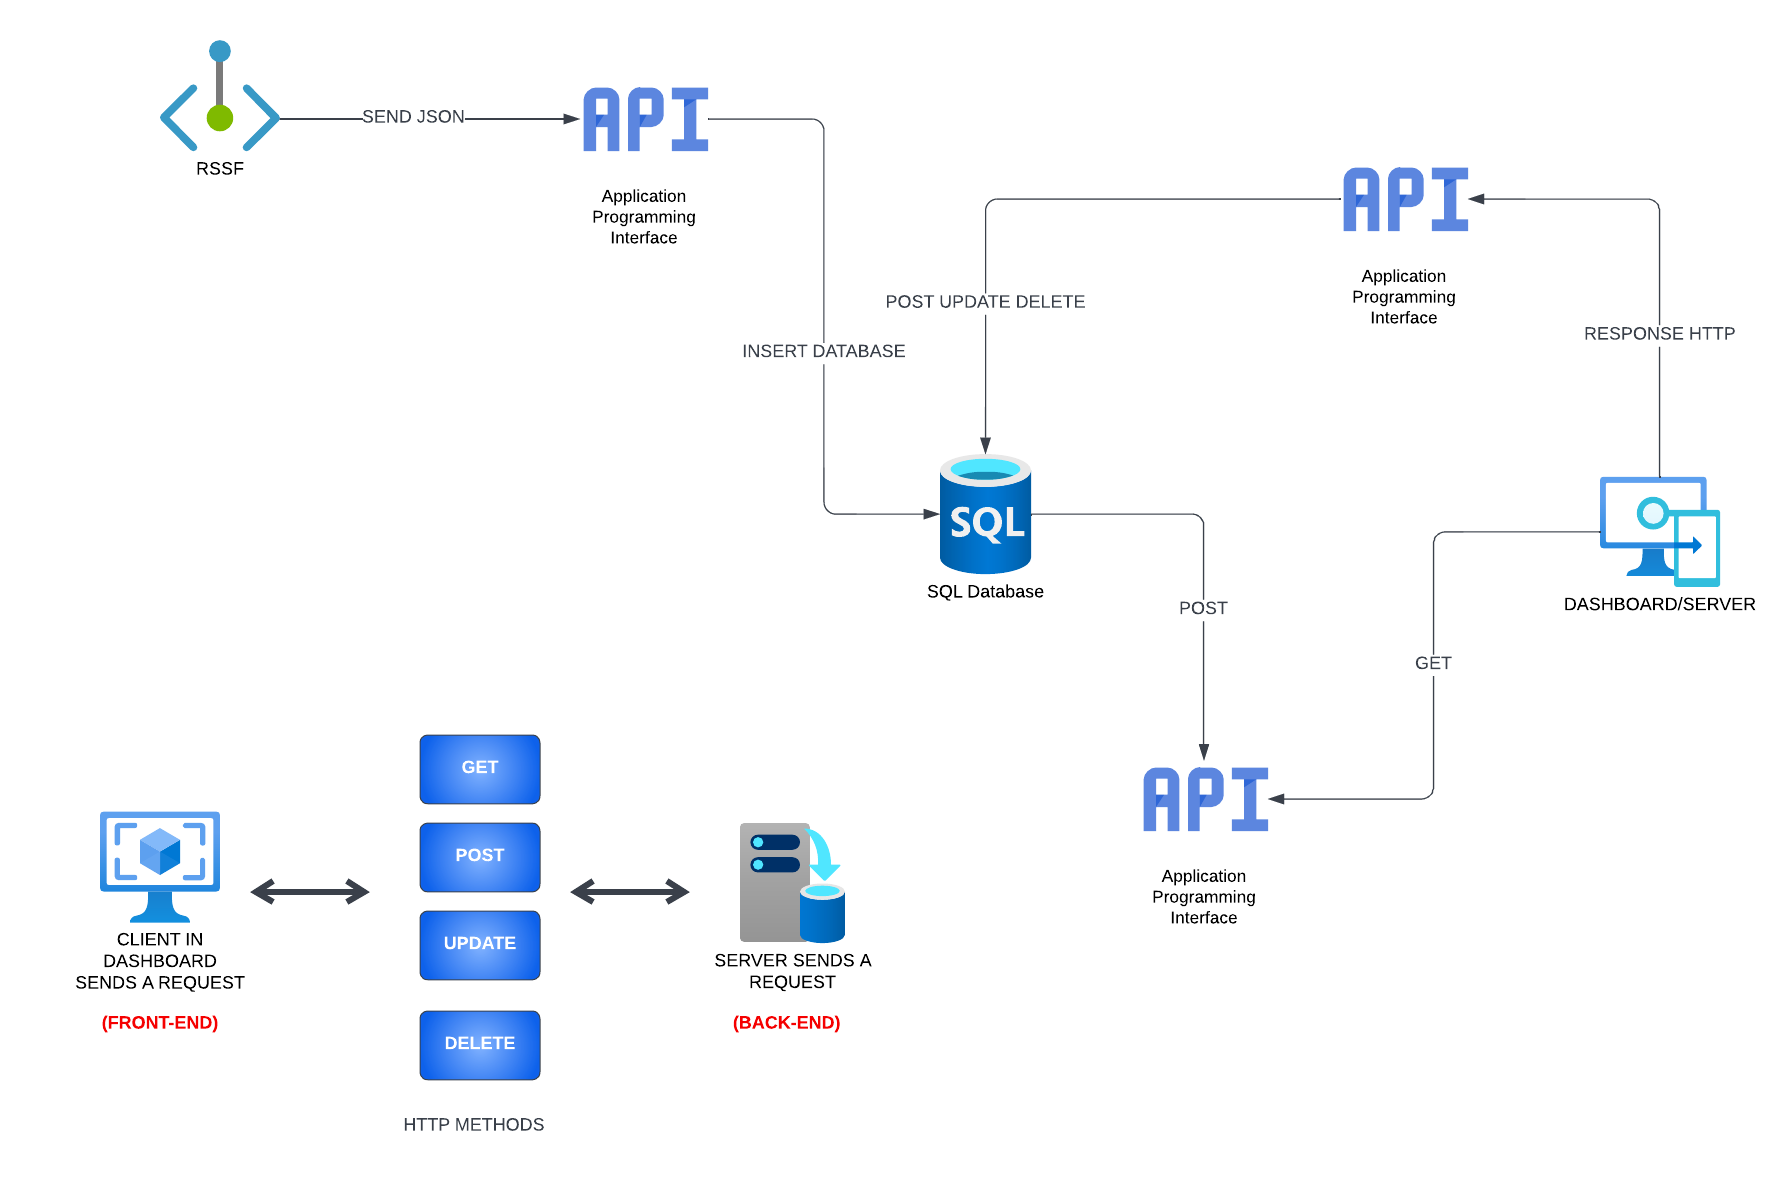
\includegraphics[scale=0.6]{tcc_flowchart.png}
    \caption{Fluxograma básico do sistema}
    \label{fig:my_label}
\end{figure}

Em geral, o resumo do objetivo deste trabalho é implementar um sistema de informação web, mais conhecido como software web, que roda diretamente no navegador, sendo assim disponível em qualquer dispositivo, sendo ele desktop, tablet ou mobile, com um formato de conexão via internet para receber os dados dos sensores localizados em campo, armazená-los em um banco de dados, dispondo de ferramentas de análise de dados para extrair informações dos dados recebidos e, por fim, permitir a visualização dos dados em formato de \textit{dashboards} com o intuito de melhorar a compreensão do usuário e viabilizar o desenvolvimento de sistemas de recomendação e a realização das análises preditivas.
\\

Através de ferramentas de Engenharia de Software, Banco de Dados, técnicas de Análise de Dados e conceitos de Experiência de Usuário podemos integrar à plataforma uma conexão segura com os componentes de hardware utilizando a internet como forma de comunicação, podendo fornecer informações visuais em formato de gráficos para o usuário final.
\\

Para alcançá-los, os seguintes objetivos específicos se fazem necessários:
\begin{enumerate}

\item Criação das APIs para comunicação dos dados entre os sensores, o banco de dados e a plataforma web.
\item Conhecimento dos processos de desenvolvimento, manutenção, metodologias ágeis e estratégias específicas para testes e customizações do sistema.
\item Desenvolvimento de um CRUD para manipulações de registros realizadas diretamente no banco de dados com o intuito de estabelecer o modelo correto no manuseio desses dados.
\item Implementação de um modelo preditivo para extração de informações valiosas de dados históricos gerados pelos sensores com o intuito de decidir as melhores ações que possam prever possíveis cenários.
\item Definição dos ciclos de vida, propondo também uma documentação adequada aos parâmetros dos modelos de qualidade de software MPS-BR nível G.
\end{enumerate}







%do Projeto. Os objetivos não devem ser confundidos com as
%atividades. Para a definição das atividades, deve-se partir dos
%objetivos determinados nesta seção. O objetivo Geral do Projeto
%necessariamente deve ser algum resultado prático (implementação) ou
%teórico (modelos formais ou especificações ou validações) produto da
%pesquisa realizada no período de Projeto de Conclusão de Curso. Assim
%como os objetivos específicos, que são considerados como subprodutos
%do Objetivo Geral.

\chapter{Metodologia}
O primeiro passo será a análise de requisitos, para obter uma visão mais detalhada do projeto, visando identificar, ainda nesta fase, funcionalidades que podem se mostrar incompletas, ambíguas ou até mesmo contraditórias dentro do sistema de informação proposto. Segundo a ~\citet{IEEE:1990} a análise de requisitos é um processo que envolve o estudo das necessidades do usuário para se encontrar uma definição correta ou completa do sistema ou requisito de software. Essa etapa será de suma importância para o desenvolvimento, pois os requisitos coletados fornecerão a referência para validar a aplicação. Serão realizadas reuniões periódicas com o grupo atuante no projeto de pesquisa que este trabalho se enquadra, de forma a compreender as finalidades do sistema, bem como, os tipos de dados e informações enviadas pelos sensores, sendo vital para a conclusão deste, a comunicação entre os integrantes da pesquisa, visto que, uma etapa está conectada a outra.
\\

Após consolidarmos os requisitos da aplicação, a próxima etapa envolverá a modelagem, onde serão feitos o planejamento em forma de fluxogramas do funcionamento, contendo os diagramas de casos de uso, classe e sequência. Dessa forma, podemos compreender o comportamento requerido do sistema a partir da perspectiva do usuário final. Também será implementada nesta etapa a criação do diagrama entidade relacionamento e o modelo lógico com o objetivo de facilitar o projeto do banco de dados neste sistema de informação possibilitando especificar a sua estrutura lógica. Além disso, neste estágio será definido a linguagem de programação e as ferramentas que serão utilizadas para o desenvolvimento. Com isso já será possível visualizar o sistema como ele é ou como desejamos que se torne ao final da construção.
\\

Na etapa de implementação, ou o desenvolvimento prático do sistema, é que começaremos a escrever, de fato, o código de programação, com base na modelagem e nos requisitos da etapa anterior. Nesta etapa daremos início a criação da interface do sistema, tal como a página de login, o registro de usuários da aplicação, a criação das APIs que vão integrar os dados do sensores, a criação dos gráficos em formato de dashboard para o usuário final e a implementação de modelos preditivos para extração de informações valiosas de dados históricos gerados pelos sensores. É bem provável que, o desenvolvimento deste sistema de informação contará com o apoio de ferramentas para agilizar o processo de desenvolvimento, como bibliotecas ou \textit{frameworks} que nos permitirão aproveitar as funções que já foram desenvolvidas, eliminando a necessidade de implementação, a exemplo disso, é esperado o uso de uma biblioteca para a criação dos gráficos. Destaca-se que essa poderá ser uma das etapas mais longas do ciclo de desenvolvimento, pois refinamentos para correções de erros são comumente necessários.
\\

Para verificarmos a eficiência e o bom funcionamento do sistema que este trabalho propõe, devemos passar por uma fase de teste, para testar a funcionalidade, o desempenho e a usabilidade. Nas partes funcionais daremos prioridade aos testes de navegação e as interações do usuário, dessa forma testaremos se as páginas estarão funcionando corretamente, a exemplo de conseguir cadastrar usuários e sensores corretamente, efetuar login, e o funcionamento correto das rotas entre as páginas e os links. 
\\

No que se refere à desempenho, testaremos as partes não funcionais do sistema como: transferência de dados, o uso de largura de banda da rede, o máximo de usuários simultâneos, a utilização de memória, a eficiência da carga de trabalho e tempos de resposta aos comandos. Vale frisar a importância do ponto de vista da qualidade para o uso da plataforma pelo usuário, uma vez que, se o produtor rural que é o usuário final neste caso quiser baixar um relatório com as informações de determinado sensor e o tempo de resposta da aplicação for muito alta, o desempenho da aplicação não será proveitoso. Caso contrário, se o sistema atender aos requisitos de desempenho poderá ser útil testar a performance com até mil (1.000) usuários simultâneos, por exemplo.
\\

Quanto a usabilidade, serão testadas as partes que envolvem a experiência do usuário ao utilizar o sistema, ou seja, qual será a facilidade de usabilidade do sistema. Para isso, poderemos testar a responsividade para diversos dispositivos, assim como os conceitos de UI/UX para o fácil manejo do sistema. Ao final dos testes o sistema passará por uma validação através de dois estudos de caso, com o intuito de checarmos se as informações que serão enviadas pelos sensores conferem com as projeções da aplicação proposta neste trabalho.
\\

Por fim, adentraremos na etapa da documentação que é fundamental para que possamos manutenir o sistema. Essa parte é de extrema importância para o futuro da aplicação, levando em consideração que este projeto vai além de um trabalho de conclusão de curso, podendo se manter no mercado, e ajudar os próximos desenvolvedores que não estiveram envolvidos com o processo de desenvolvimento a compreenderem melhor o projeto em si. Em geral, para a documentação de sistemas de informação web será de suma relevância a descrição de quais páginas usam determinados arquivos, e também a referenciação das APIs que poderá ser feita de forma manual ou utilizando ferramentas, visto que documentá-las detalhadamente economizará tempo e custos de suporte.

%Nesta seção, apresenta-se a metodologia proposta para o
%desenvolvimento do Projeto. O proponente do Projeto deve descrever
%superficialmente as atividades necessárias para a conclusão dos
%objetivos propostos, normalmente utilizando um parágrafo para cada
%objetivo.

\chapter{Plano de Atividades e Cronograma}
% (PARA 1 ANO)

\begin{center}
\begin{tabular}{ | m{3.6cm} | m{0.65cm}| m{0.65cm} | m{0.65cm} | m{0.65cm} | m{0.65cm} | m{0.65cm} | m{0.65cm} | m{0.65cm} | m{0.65cm} | m{0.65cm} | m{0.65cm} | m{0.65cm} | m{0.65cm} | } 
  \hline
   Tarefa & Ago & Set & Out & Nov & Dez & Jan & Fev & Mar & Abr & Mai & Jun & Jul  \\ 
  \hline
  Análise de Requisitos & X & X & & & & & & & & & & \\
  \hline 
  Revisão da bibliografia & X & X & X & X & X & X & X & X & X & X & &\\
  \hline
  Escrita da Monografia Parcial & & X & X & & & & & & & & & \\
  \hline
  Entrega da Monografia Parcial & & & & X & & & & & & & & \\
  \hline
  Modelagem do Sistema & & X & X & & & & & & & & & \\
  \hline
  Implementação & & & X & X & X & X & X & X & X & & & \\
  \hline
  Escrita da Monografia Intermediária & & & & X & X & X & & & & & & \\
  \hline
  Entrega da Monografia Intermediária & & & & & & & X & & & & & \\
  \hline
  Testes e Validação & & & & & & & & & & X & X & \\
  \hline
  Escrita da Monografia Final & & & & & & & X & X & X & X & X & \\
  \hline
  Manutenção e Documentação & & & & & & & & & & & X & X\\
  \hline
  Preparação para defesa do TCC & & & & & & & & & & & X & \\
  \hline
  Defesa do TCC e entrega da Monografia Final & & & & & & & & & & & & X \\
  \hline
\end{tabular}
\end{center}


\bibliography{bibliografia}
\bibliographystyle{abnt}

\chapter{Assinaturas}
\vspace{2cm}

\begin{center}
\rule{8cm}{.3mm}
\medskip

	Coloque aqui o seu nome\\
	Proponente

\end{center}

\vspace{4cm}

\begin{center}
\rule{8cm}{.3mm}
\medskip

	Coloque aqui o nome do professor\\
	Prof. Orientador

\end{center}
\end{document}

